\documentclass[11pt,reqno]{amsart}
\usepackage{amsfonts,amssymb,amscd,amsmath,mathrsfs,amsthm}
\usepackage[pdftex]{graphicx}

\setlength{\oddsidemargin}{0.25in}  %please do not change
\setlength{\evensidemargin}{0.25in} %please do not change
\setlength{\marginparwidth}{0in} %please do not change
\setlength{\marginparsep}{0in} %please do not change
\setlength{\marginparpush}{0in} %please do not change
\setlength{\topmargin}{0in} %please do not change

\setlength{\footskip}{.3in} %please do not change
\setlength{\textheight}{8.75in} %please do not change
\setlength{\textwidth}{6in} %please do not change
\setlength{\parskip}{4pt} %please do not change

%
% The following lines set the environments for theorems, propositions, and definitions. 
%

\theoremstyle{plain}
\newtheorem{thm}{Theorem}[section]
\newtheorem{prop}{Proposition}

%  Alternatively, can use
%  \newtheorem{thm}{Theorem}[section]
%  to create theorems with numbering depending on the sections.
%
%  \newtheorem{prop}[thm]{Proposition} will generate propositions that use the same counter as theorems.

\theoremstyle{definition}
\newtheorem*{defi}{Definition}


\newcommand{\ab}[2]{\left(\frac{#1}{#2}\right)}

%  Mathematical sets; R, C, ...

\begin{document}

\section{Graphics}


 The package to load is \textbackslash{}usepackage[pdftex]\{graphicx\}. The command includegraphics' loads a file, in this case example.pdf. Replace with your own file.
 
 The file needs to be in the same directory as the latex file.
  An easy way to generate plots is to use Mathematica, see code on blackboard.
The different options for the `figure' environment are listed in the latex guide
 on blackboard, same with the options for `includegraphics'.

\begin{figure}[h]
\begin{center}
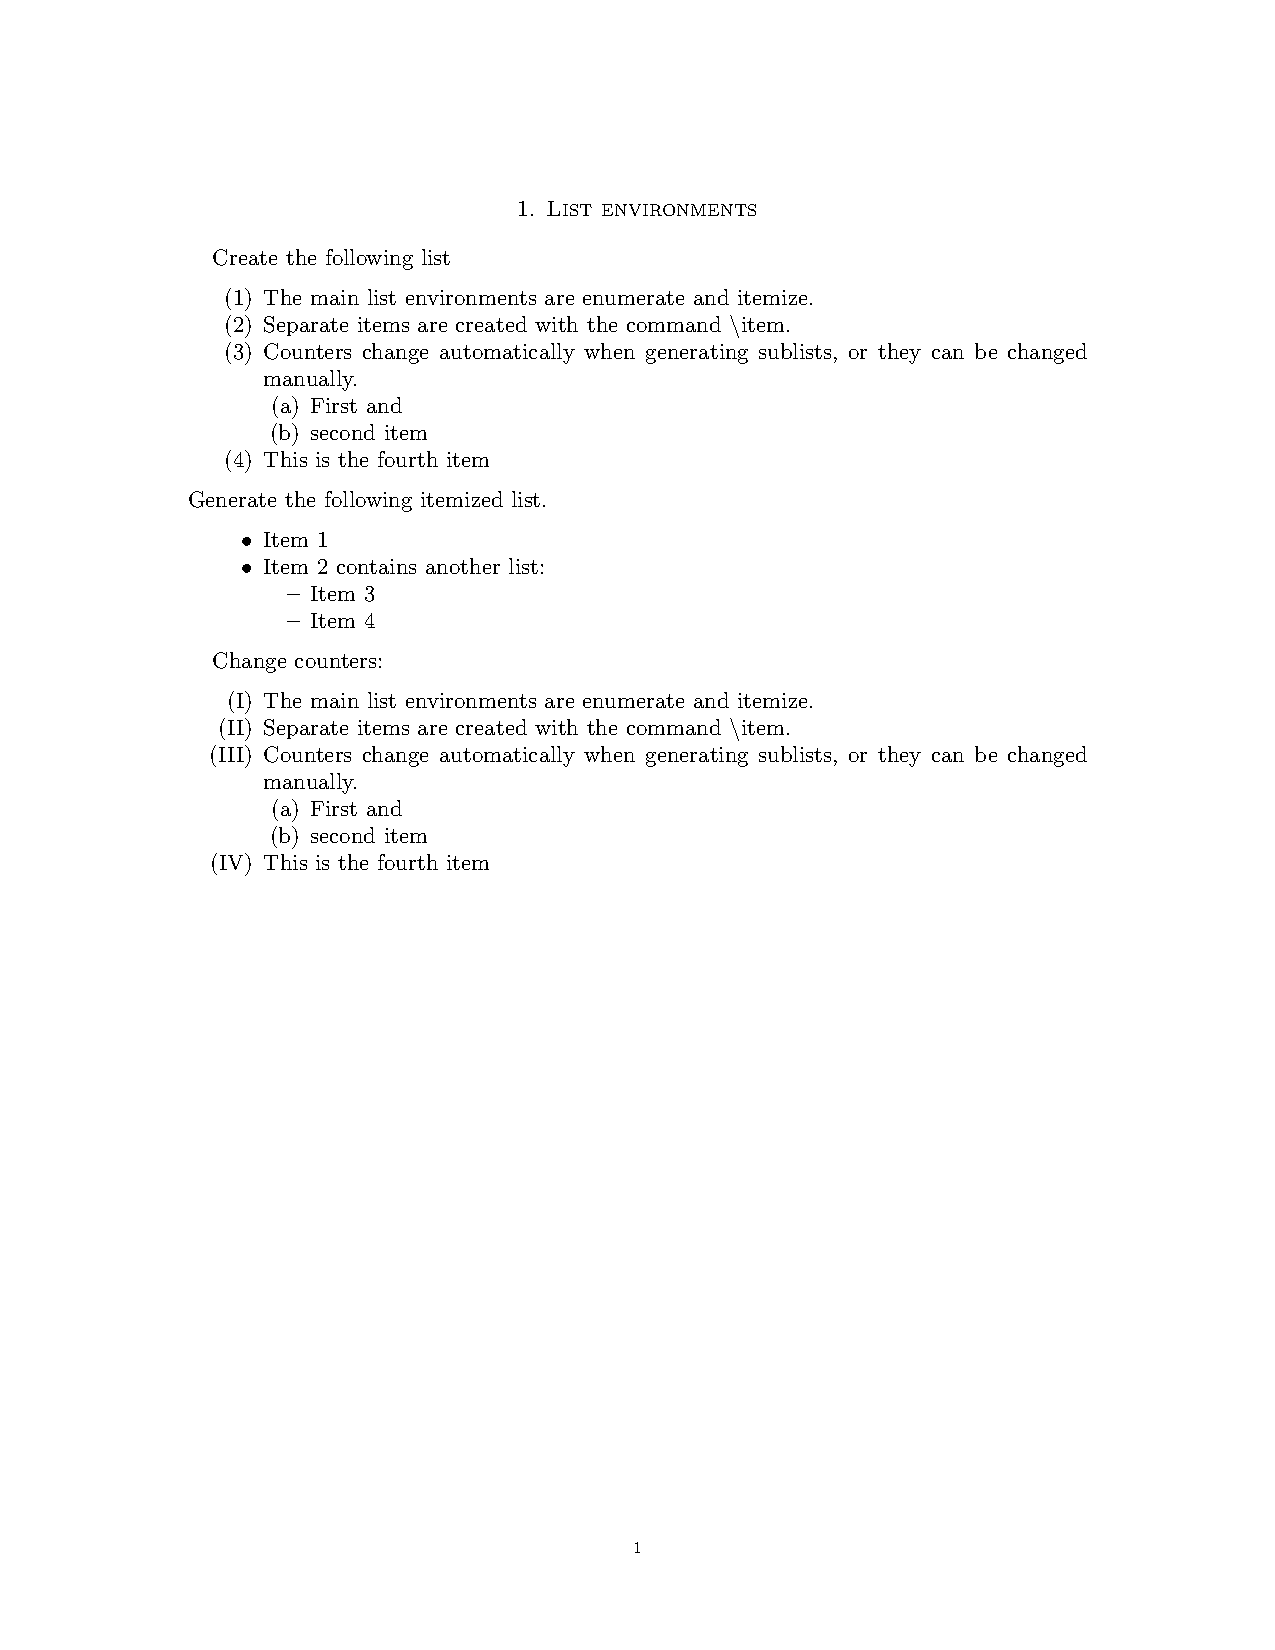
\includegraphics[width=7cm]{script4math}
\caption{A simple graph}
\end{center}
\end{figure}


\end{document}
